\documentclass[11pt]{article}

\usepackage[a4paper,margin=2.6cm]{geometry}
\usepackage[T1]{fontenc}
\usepackage{lmodern}
\usepackage{microtype}
\usepackage{amsmath,amssymb,mathtools}
\usepackage{booktabs,longtable,tabularx,array}
\usepackage{graphicx}
\usepackage{tikz}
\usetikzlibrary{arrows.meta,positioning,fit,calc,shapes.geometric}
\usepackage[backend=biber,style=authoryear,natbib=true,maxcitenames=2,maxbibnames=20]{biblatex}
\addbibresource{references.bib}
\usepackage[hidelinks]{hyperref}
\usepackage[nameinlink,noabbrev]{cleveref}
\usepackage{xcolor}
\usepackage{enumitem}
\usepackage{setspace}

\newcommand{\V}{\mathcal V}
\newcommand{\D}{\mathcal D}
\newcommand{\A}{\mathcal A}
\newcommand{\Mvec}{\mathbf M}
\newcommand{\R}{\mathbb R}
\newcommand{\dd}{\,\mathrm d}
\newcommand{\claimstatus}[1]{\textsc{#1}}

\title{\textbf{From Distributed Control to Distributed Maintenance}\\
\large Boundary Conditions for Viability in Decentralized Systems}
\author{Albert Jan van Hoek}
\date{Draft --- September 2026}

\begin{document}
\maketitle

\begin{abstract}
Many systems persist without a central controller. Cells maintain physiological conditions through distributed regulation; fungal networks remodel transport pathways; ecological networks preserve functions through interacting populations; and engineered protocols rely on distributed participants to detect and correct failure. These systems differ radically in substrate, yet they share a problem: the processes that maintain collective viability are themselves local, fallible, resource-dependent, and embedded in the system they regulate.

This paper develops a cross-substrate framework for analysing such \emph{distributed maintenance}. The framework does not propose a new theory of feedback control, viability, organizational closure, or biological regulation. Instead, it synthesizes a sequence of boundary conditions that become visible when local control is distinguished from system-level continuation. We show why several apparently natural inferences fail: locally selected control need not be sufficient for viability; persistence need not demonstrate present self-maintenance; participant presence need not imply positive contribution; identical present states can conceal different corrective capacities; and a process can be reinforced even when the signal driving its reinforcement has become decoupled from the function whose continuation matters. In systems with several continuation requirements, contribution is naturally vector-valued and need not possess a weight-independent global sign.

We formalize these observations using a declared viability region, disturbance class, distributed maintenance architecture, and multiple admissibility constraints. This yields a conservative interpretation of an ``ought'': given a dynamical model and a stipulated continuation criterion, parameters or actions must remain in an admissible region if that criterion is to continue. The logical sequence is therefore \emph{model $\rightarrow$ viability-conditioned requirement $\rightarrow$ observation $\rightarrow$ practical response}, rather than an attempt to derive categorical norms from persistence.

JAM/ELVES-style distributed verification and adaptive fungal transport are used as contrasting worked examples. Their value lies not in demonstrating identical mechanisms, but in identifying which descriptions survive large changes of substrate. The resulting framework treats distributed maintenance as a network of processes linking viability-relevant function, informative coupling, corrective action, renewal, independent capacity, and revision. It generates a set of empirical tests for distinguishing merely persistent systems from systems whose current organization is actively maintaining the conditions of future viability.
\end{abstract}

\section{Introduction}

A system that exists at time \(t\) has survived until time \(t\). Much less follows from that statement than is often assumed.

Its present condition may have been inherited from earlier activity rather than generated by current processes. A currently functioning system may be consuming reserves faster than it replaces them. A participant that appears useful in isolation may reduce collective viability once network responses are considered. A regulator that is individually favoured may provide less control than the wider system requires. A signal used to reinforce a process may gradually cease to measure the function for which the process was originally retained.

These are not unusual exceptions. They arise whenever the processes responsible for maintaining an organization are distributed across interacting components with different incentives, time scales, dependencies, signals, and failure modes.

The relevant question is therefore not merely: \emph{What state is the system currently in?} Nor even: \emph{Which components contribute to that state?} The stronger question is:

\begin{quote}
\textbf{Which current processes maintain the capacity of the system to remain within its declared viability conditions under future disturbance, and what maintains those processes themselves?}
\end{quote}

This question connects several mature traditions.

Viability theory studies whether dynamical systems can remain within specified constraint sets and characterizes the states and controls from which continued viability is possible \citep{aubin1991,aubin2011}. Organizational approaches to biology describe organisms as networks of mutually dependent constraints that participate in one another's production and maintenance \citep{mossio2010,montevil2015,moreno2015}. Di Paolo's account of adaptivity links regulation to conditions of viability and organism-relative normativity \citep{dipaolo2005}. Bich and colleagues characterize biological regulation as a form of second-order control that modulates constitutive processes in response to perturbation \citep{bich2016}; subsequent work emphasizes heterarchically organized control rather than necessarily centralized control \citep{bich2022}.

The present paper does not replace these theories. Its narrower purpose is to connect them to a recurring problem exposed by a sequence of formal and computational models of distributed regulation: \emph{the variables that describe current organization are not sufficient to describe the processes that maintain the future possibility of that organization}.

The synthesis developed here is built around boundary conditions rather than a claim of successive scientific falsifications. Each modelling exercise exposed a point at which the previous representation ceased to be sufficient. Several resulting mathematical statements are elementary, and several recover known principles from reliability engineering, control theory, cooperation research, viability theory, and adaptive-network theory. Their value here is compositional: taken together, they suggest a diagnostic framework for distributed maintenance.

The central proposal is
\begin{center}
\fbox{\parbox{0.88\linewidth}{\centering
Distributed maintenance concerns the preservation of viability-relevant
relations and capacities, not merely the persistence of present state.}}
\end{center}

This leads to six separations:
\[
\begin{aligned}
\text{local selection} &\not\Rightarrow \text{sufficient control},\\
\text{persistence} &\not\Rightarrow \text{present self-maintenance},\\
\text{presence} &\not\Rightarrow \text{positive contribution},\\
\text{state} &\not\Rightarrow \text{corrective capacity},\\
\text{reinforcement signal} &\not\Rightarrow \text{viability-relevant function},\\
\text{one positive contribution} &\not\Rightarrow \text{global benefit}.
\end{aligned}
\]

The paper asks what survives once these implications are removed.

\section{Relation to the preceding programme}

The framework developed here should not be read as re-presenting several results already developed in companion work.

\subsection{Persistence does not measure function}

\emph{Persistence Does Not Measure Function} separates equilibrium persistence, productive efficiency, maintained mass, structural support, and externally specified functional capacity \citep{vanhoek2026persistence}. Its counterexamples show that a system can improve according to one of these quantities while deteriorating according to another.

The present paper takes that separation as given. It asks what additional variables are needed once the object of study becomes the \emph{maintenance of future viability} rather than present function alone.

\subsection{Selected regulation does not guarantee sufficient regulation}

\emph{When Does Regulation Pay?} distinguishes the controller strength selected under a stated endogenous objective from the strength required to satisfy an independently declared functional condition \citep{vanhoek2026regulation}. In its minimal model,
\[
k_{\rm opt}\neq k_{\rm func}
\]
in general, and regulation may be retained while remaining too weak to satisfy the functional boundary.

The present paper does not reclaim this as a new result. Instead it generalizes the inferential lesson:
\[
\boxed{
\text{the process selected locally need not supply the quantity required collectively.}
}
\]

\subsection{Present persistence does not establish present maintenance}

A separate test programme distinguishes current stock from the current processes replacing loss and restoring disturbances \citep{vanhoek2026present}. A system can therefore appear healthy while inherited capacity is being depleted.

Again, the present paper takes this result as a starting condition. Its added question is how such maintenance is distributed across a network, how individual contributions depend on architecture and state, and how the maintenance processes themselves persist.

Thus the present manuscript is not a replacement for these companion papers. It is a synthesis of the boundary conditions that become visible when their distinctions are applied to decentralized organization.

\section{Claim-status map}

Because this manuscript combines prior art, results established elsewhere in the author's programme, exact consequences of declared toy models, and new synthesis, those categories are kept explicit throughout. \Cref{tab:claims} summarizes the status of the main claims.

\begin{table}[htbp]
\centering
\small
\caption{Claim-status map. ``Exact model result'' means exact within the stated model; it does not imply empirical validation or literature priority.}
\label{tab:claims}
\begin{tabularx}{\textwidth}{@{}p{0.05\textwidth}X p{0.21\textwidth}@{}}
\toprule
ID & Claim & Status \\
\midrule
S1 & Persistence, productive efficiency, maintained mass, structural support, and functional capacity need not coincide. & \claimstatus{previous paper} \\
S2 & Locally selected regulatory strength need not be sufficient for an independently declared functional boundary. & \claimstatus{previous paper} \\
S3 & Present state does not in general identify present corrective or renewal capacity. & \claimstatus{previous work + exact model} \\
S4 & Participant contribution is relational: its sign can change after network response or across viability criteria. & \claimstatus{exact model / established analogue} \\
S5 & In sampled or capacity-limited correction, participant addition can alter causal access to correction; all-participant monotonicity does not automatically transfer. & \claimstatus{JAM companion paper} \\
S6 & Mixed-sign effects across several viability margins have no weight-independent global scalar sign. & \claimstatus{elementary exact result} \\
S7 & Corrective capacity that decays or is consumed must itself receive sufficient renewal if it is to persist. & \claimstatus{elementary exact result / prior art} \\
S8 & A signal used to allocate renewal can diverge from the viability-relevant function it is meant to track. & \claimstatus{new synthesis / hypothesis} \\
S9 & ``Function--renewal proxy gap'' is proposed as a diagnostic variable for that divergence; no universal metric is claimed. & \claimstatus{new terminology} \\
S10 & A distributed maintenance architecture can be represented as viability specification, informative coupling, response, independent corrective capacity, return, capacity renewal, and architectural revision. & \claimstatus{proposed synthesis} \\
S11 & Viability-conditioned requirements have the form model + declared viability property \(\Rightarrow\) admissible region; they are not categorical moral obligations. & \claimstatus{viability-theory interpretation} \\
S12 & The framework earns empirical value only if its explicit maintenance variables improve prediction or intervention beyond state-only or trend-only models. & \claimstatus{test criterion} \\
\bottomrule
\end{tabularx}
\end{table}

\section{A minimal language of distributed viability}

Let the system state at time \(t\) be \(z_t\in Z\). Let its dynamics be
\[
\boxed{
z_{t+1}=F(z_t,\theta,d_t),
}
\]
where \(\theta\) describes architecture, control parameters or policies; \(d_t\in\D\) is a disturbance; and \(\D\) is the declared disturbance class.

Let
\[
\V\subseteq Z
\]
denote a declared viability region. The one-step admissible region is
\[
\boxed{
\A_{\V}(z)
=
\left\{
\theta:
F(z,\theta,d)\in\V
\quad
\forall d\in\D
\right\}.
}
\]
Longer-horizon viability asks whether some admissible policy keeps the resulting trajectory within \(\V\). This is standard territory for viability and invariance theory.

The new terminology introduced here concerns the architecture implementing those admissible dynamics.

\paragraph{Definition (distributed maintenance architecture).}
A \emph{distributed maintenance architecture} is a collection of local processes whose state-dependent actions jointly alter the probability or margin by which one or more declared viability conditions will continue to hold.

This definition deliberately does not require autonomous agents, explicit rewards, conscious goals, centralized monitoring, biological individuality, or a single scalar system objective. The word \emph{maintenance} therefore refers to a functional relation between present processes and future viability, not to a particular mechanism.

\section{From state to margin}

Membership in \(\V\) is often too coarse for studying maintenance. We therefore introduce a viability margin
\[
M(z,\theta),
\]
where \(M>0\) denotes remaining room before a declared boundary is crossed, \(M=0\) the boundary itself, and \(M<0\) failure of that particular criterion.

The exact definition is application-specific. For a simple stock \(K\) with viability threshold \(V\),
\[
M=K-V.
\]
For a distributed verification system it might be a log safety-certificate margin. For a population it might be distance from a transmission or extinction boundary.

For several simultaneous requirements, define
\[
\boxed{
\Mvec=(M_1,\ldots,M_k).
}
\]
This apparently modest change matters because a distributed process can affect different viability margins in opposite directions. The system therefore need not admit a natural scalar statement of ``better.''

\section{Boundary condition I: selected control is not sufficient control}

Suppose individual process \(i\) chooses effort \(a_i\) according to a local objective \(U_i(a_i,z)\). Let \(a_i^{\rm sel}\) denote a locally selected action, while collective viability requires
\[
a\in\A_{\V}(z).
\]
Nothing in optimization guarantees
\[
a^{\rm sel}\in\A_{\V}(z).
\]

This is not peculiar to biological selection or economic incentives. It is a general mismatch between two optimization problems:
\[
\boxed{
\text{what persists locally}
\quad\text{and}\quad
\text{what suffices globally}.
}
\]
This distinction was the organizing result of the companion regulation paper and also appears in the initial distributed-control models.

Its importance for distributed maintenance is methodological. Observing that a behaviour is stable, common, rewarded, individually rational, evolutionarily retained, or protocol-compatible does not establish that it supplies enough of the function required by the wider system. The viability requirement must be specified independently.

\section{Boundary condition II: participant presence is not participant contribution}

Distributed systems tempt us to treat the existence of a component as evidence of its contribution. But contribution is a counterfactual relation.

For participant \(i\), architecture \(A\), state \(z\), and viability component \(j\), write
\[
\boxed{
C_{ij}(z,A)
=
M_j(z',A')
-
M_j(z,A),
}
\]
where the first term represents a declared counterfactual in which participant \(i\) is added, removed, modified, or reassigned and all relevant downstream consequences are included.

The notation intentionally leaves the counterfactual specification explicit. Different attribution schemes answer different questions. A leave-one-out calculation asks whether \(i\) is currently necessary. A Shapley allocation asks about average marginal contribution over coalition orderings. An interaction decomposition asks where non-additivity resides. None is a universal measure of intrinsic value.

\subsection{Contribution depends on network response}

A participant can have a positive direct effect but a negative post-adjustment effect if other processes re-equilibrate in response. Thus
\[
C_i^{\rm direct}>0
\]
does not imply
\[
C_i^{\rm equilibrium}>0.
\]

This is familiar in ecological interaction networks, economics and game theory, but it is a crucial safeguard for any theory of distributed maintenance. Contribution belongs to a relation:
\[
\boxed{
\text{participant}
\times
\text{network state}
\times
\text{architecture}
\times
\text{viability criterion}.
}
\]

\subsection{Sampling adds another architecture dependence}

A companion analysis of JAM/ELVES develops an important engineered instance in detail: when correction is supplied by all available participants, adding another corrective participant is structurally monotone; when correction is allocated through a constrained sample, addition can alter which other corrective processes gain access to the sample.

The synthesis point is broader:
\begin{center}
\fbox{\parbox{0.88\linewidth}{\centering
Contribution depends not only on what a participant can do,
but on how the architecture gives it causal access to the relevant function.}}
\end{center}
The technical JAM result belongs in the companion protocol paper; here it serves only as evidence that the architecture must be part of the definition of contribution.

\section{Boundary condition III: present state is not corrective capacity}

Two systems can occupy the same visible state while possessing very different abilities to survive the next disturbance.

Let \(X_t\) denote present performance or shared state and \(C_t\) a slower stock of corrective capacity. A minimal shock model is
\[
X_{\rm after}=X-s+\kappa C,
\]
with viability condition
\[
X-s+\kappa C\ge V.
\]
The corresponding disturbance margin is
\[
\boxed{
M(X,C)=X-V+\kappa C.
}
\]
At fixed \(X\),
\[
\frac{\partial M}{\partial C}=\kappa.
\]

Hence two systems can have identical observed performance, \(X_1=X_2\), while \(C_1\neq C_2\) gives \(M_1\neq M_2\).

This is elementary algebra, but it exposes a major diagnostic problem. A system may look stable because it has not yet been challenged. Or it may look stable because substantial corrective machinery exists but remains dormant. Those states are observationally similar under quiet conditions and dynamically different under disturbance.

Therefore:
\[
\boxed{
\text{current state is not a sufficient statistic for future viability.}
}
\]

\section{Boundary condition IV: maintenance capacity must itself be maintained}

Corrective capacity is not automatically permanent. Consider
\[
C_{t+1}=(1-\delta)C_t+R_t,
\]
where \(R_t\) denotes renewal of capacity. At a required capacity \(C=V_C\),
\[
V_C\le(1-\delta)V_C+R
\]
is equivalent to
\[
\boxed{
R\ge\delta V_C.
}
\]

This replacement condition is almost definitional. Its importance lies not in mathematical novelty but in recursion. Once a process is necessary for maintaining another variable, its own replacement and renewal become part of the viability problem:
\[
\text{maintained state}
\leftarrow
\text{corrective process}
\leftarrow
\text{corrective capacity}
\leftarrow
\text{capacity renewal}.
\]

This resembles the organizational closure described in biological autonomy theory, where constraints participate in the production and maintenance of other constraints. Biological regulation has likewise been characterized as second-order control because it modulates constitutive processes rather than merely acting on an external target \citep{bich2016}. The present framework does not claim this recursion as new. Its extension is to use the same bookkeeping in systems that need not be organisms and need not realize organizational closure in the biological sense.

\section{Boundary condition V: the signal receiving renewal is not necessarily the function that matters}

A process can persist because something causes resources, structure, opportunity or reward to return to it.

Let \(F_i\) denote the function of process \(i\) that contributes to a declared viability condition. Let \(Y_i\) denote the locally available signal that actually drives reinforcement or renewal. Let
\[
R_i=G(Y_i)
\]
be the resulting return.

The maintenance loop is then
\[
\boxed{
F_i
\longrightarrow
Y_i
\longrightarrow
R_i
\longrightarrow
C_i
\longrightarrow
F_i'.
}
\]

A common but unsafe simplification is \(Y_i=F_i\). In many real systems, \(Y_i\) is only a proxy. The important question is therefore not simply whether a return loop exists, but whether the return-driving signal remains sufficiently informative about the function whose continuation matters.

\subsection{A function--renewal proxy gap}

We use \emph{function--renewal proxy gap} as a diagnostic term for the mismatch between \(F_i\) and \(Y_i\).

No universal scalar measure is proposed. Depending on the system, the gap could be operationalized by classification error, conditional mutual information, predictive loss, calibration error, causal intervention, or the difference between function-conditioned and proxy-conditioned return.

The important structural possibility is
\[
Y_i\uparrow
\quad\text{while}\quad
F_i\downarrow.
\]
Then the system can increasingly reinforce a process whose actual viability contribution is deteriorating. This creates a general route to lock-in.

\subsection{Engineered illustration}

In distributed verification, a positive judgment is not logically identical to having performed independent expensive verification. The architecture therefore faces a discrimination problem:
\[
\text{performed useful verification}
\neq
\text{observable evidence rewarded as verification}.
\]
If the latter becomes cheap to imitate, return may detach from function. The detailed incentive implications are protocol-specific and are not established here.

\subsection{Biological illustration}

Adaptive transport networks provide a very different implementation. In fungal mycelial networks, growth-induced flow can contain information about the network role of a cord, and cords predicted to carry larger or faster flows are more likely to increase in size \citep{heaton2010}. But current flow is also partly a consequence of existing structure. Thus
\[
\text{existing conductance}
\rightarrow
\text{flow}
\rightarrow
\text{further reinforcement}
\]
can create path dependence.

Similar flux-reinforcement mathematics is established in adaptive transport models such as \emph{Physarum} networks \citep{tero2007}. The point here is therefore not that a sublinear-versus-superlinear reinforcement threshold is new. The cross-substrate lesson is different:
\begin{center}
\fbox{\parbox{0.88\linewidth}{\centering
The signal that allocates future structure can be informative about function
while simultaneously being endogenous to past allocation.}}
\end{center}

\section{Boundary condition VI: there is no intrinsic scalar contribution in a multi-viability system}

Real systems maintain more than one condition.

Suppose participant \(i\) changes two viability margins by
\[
\Delta\Mvec_i=(a,b)
\]
with \(a>0\) and \(b<0\). Any scalar score
\[
S_i=w_1a+w_2b,
\qquad
w_1,w_2>0,
\]
depends on the weighting. Weights can be chosen such that \(S_i>0\) or \(S_i<0\). Therefore:
\[
\boxed{
\text{mixed-sign contribution has no weight-independent global sign.}
}
\]

This prevents an important category error: replacing multiple viability requirements with an implicit scalar notion of what is ``good for the system.''

The correct object is therefore a feasible region:
\[
\boxed{
\A
=
\bigcap_{j=1}^{k}\A_j.
}
\]
Three possibilities follow: the intersection is broad; it is narrow; or it is empty. If
\[
\bigcap_j\A_j=\varnothing,
\]
then no parameter tuning inside the present architecture can satisfy all declared requirements simultaneously. The intervention must move to a higher architectural level.

\section{Distributed maintenance as a network of maintenance relations}

The preceding sections suggest a representation richer than ``controller acts on state.'' \Cref{fig:maintenance} summarizes the proposed decomposition.

\begin{figure}[htbp]
\centering
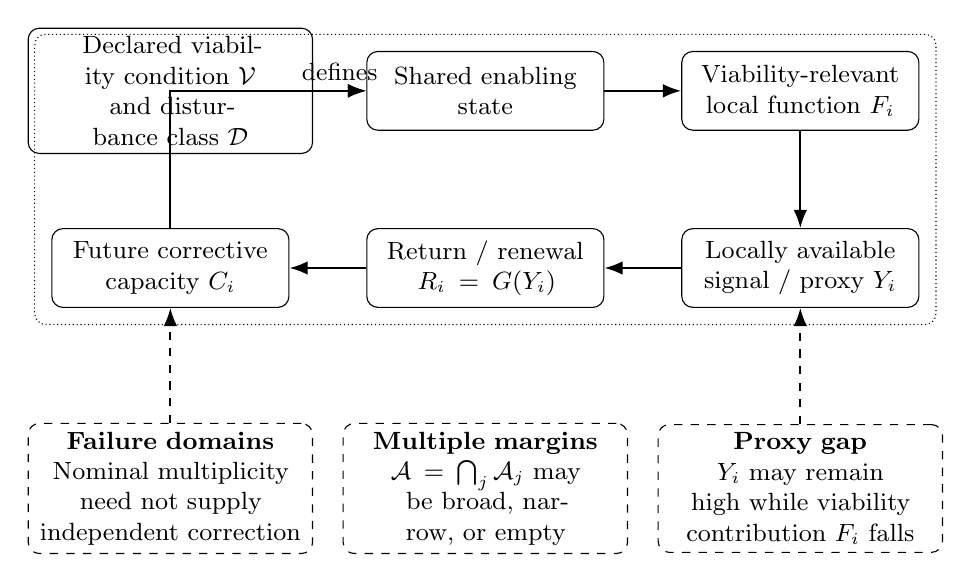
\begin{tikzpicture}[
  font=\small,
  >=Latex,
  box/.style={draw, rounded corners, align=center, minimum height=10mm, text width=28mm, inner sep=3pt},
  wide/.style={draw, rounded corners, align=center, minimum height=10mm, text width=34mm, inner sep=3pt},
  note/.style={draw, dashed, rounded corners, align=center, text width=34mm, inner sep=3pt},
  arr/.style={->, thick}
]
\node[wide] (V) at (0,3.4) {Declared viability condition \(\V\)\\and disturbance class \(\D\)};
\node[box] (S) at (4,3.4) {Shared enabling\\state};
\node[box] (F) at (8,3.4) {Viability-relevant\\local function \(F_i\)};
\node[box] (Y) at (8,1.15) {Locally available\\signal / proxy \(Y_i\)};
\node[box] (R) at (4,1.15) {Return / renewal\\\(R_i=G(Y_i)\)};
\node[box] (C) at (0,1.15) {Future corrective\\capacity \(C_i\)};

\draw[arr] (V) -- node[above]{defines} (S);
\draw[arr] (S) -- (F);
\draw[arr] (F) -- (Y);
\draw[arr] (Y) -- (R);
\draw[arr] (R) -- (C);
\draw[arr] (C.north) |- (S.west);

\node[note] (D) at (0,-1.65) {\textbf{Failure domains}\\Nominal multiplicity need not supply independent correction};
\node[note] (M) at (4,-1.65) {\textbf{Multiple margins}\\\(\A=\bigcap_j\A_j\) may be broad, narrow, or empty};
\node[note] (P) at (8,-1.65) {\textbf{Proxy gap}\\\(Y_i\) may remain high while viability contribution \(F_i\) falls};

\draw[arr,dashed] (D.north) -- (C.south);
\draw[arr,dashed] (P.north) -- (Y.south);

\node[fit=(S)(F)(Y)(R)(C), draw, densely dotted, rounded corners, inner sep=6pt] {};
\end{tikzpicture}

\caption{\textbf{Distributed maintenance as a recursive viability architecture.}
A declared viability condition specifies what continuation means under a disturbance class. Local processes receive function-relevant information, act on shared state, and depend on return or renewal for future corrective capacity. Failure-domain structure determines whether nominal multiplicity supplies independent correction. The function--renewal proxy gap appears when the signal that attracts return diverges from the function relevant to viability. Multiple viability conditions generate intersecting admissible regions rather than a single scalar objective.}
\label{fig:maintenance}
\end{figure}

For each local process, distinguish at least the following relations.

\subsection{Viability specification}

The continuation property and disturbance class must be stated. Without this step, ``maintenance'' has no definite target.

\subsection{Informative coupling}

Some local variable must carry information relevant to the condition being maintained. This need not mean representation in a cognitive sense.

\subsection{Corrective or adaptive effect}

Changes in the local process must alter future viability. Otherwise the signal is epiphenomenal with respect to the declared condition.

\subsection{Independent corrective capacity}

Where common-mode failure is possible, nominal multiplicity is not equivalent to independent correction. Reliability depends on failure topology.

\subsection{Return-loop closure}

Processes that consume resources or decay must receive sufficient renewal to continue supplying their function. The return may be metabolic, energetic, structural, reproductive, economic or informationally mediated.

\subsection{Renewal of maintenance capacity}

The ability to correct future disturbance must itself survive quiet periods, use, degradation and replacement.

\subsection{Architectural corrigibility}

The maintenance architecture can itself become maladaptive. A system able only to correct its object-level state, but unable to revise a failing maintenance mechanism, remains vulnerable to structural change outside the mechanism's operating assumptions.

These seven items are proposed as a diagnostic decomposition. They are not claimed to be universally necessary and sufficient conditions for every persistent network.

\section{Worked comparison: engineered auditing and fungal transport}

The purpose of comparing radically different substrates is not to assert mechanism identity. It is to ask what remains meaningful when obvious substrate-specific concepts are removed.

\subsection{Engineered distributed verification}

In a distributed verification protocol, one can identify a validity condition, randomly selected verification processes, explicit judgments, escalation after detectable failure, implementation diversity, fault records, and externally supplied economic return.

The architecture is highly explicit. Signals, actions and participants have designed semantics. Yet the analysis reveals that nominally honest participation is not automatically equivalent to independent corrective capacity, and that an observable output such as a judgment need not by itself establish the costly process presumed to generate it.

The companion JAM/ELVES manuscript develops those claims at protocol level. They are not repeated here as evidence of a generic theorem.

\subsection{Fungal transport}

A fungal network contains no validator, voting rule or staking contract. Its transport architecture nevertheless involves flows through network paths, local structural growth and regression, redistribution under changing resource conditions, topology-dependent transport, and trade-offs among connectivity, transport efficiency, robustness and construction cost.

Empirical work shows that fungal network traits occupy such trade-offs rather than maximizing a single objective \citep{aguilar2022}.

The useful comparison is therefore not
\[
\text{validator}=\text{fungal cord},
\]
nor
\[
\text{reward}=\text{nutrient}.
\]

The defensible cross-substrate statement is weaker:

\begin{quote}
In both systems, future allocation to a local process depends on information generated by its interaction with a wider network, and that allocation alters future network capacity.
\end{quote}

The implementation differs radically. The maintenance relation survives.

\subsection{What the comparison removes}

The comparison shows why several terms should not be primitives of the general framework: \emph{agent} is too restrictive; \emph{monitor} is too architectural; \emph{reward} is too economic; \emph{commons} is too domain-specific; and \emph{individual} may be ambiguous across scale.

More neutral terms are
\[
\boxed{
\text{local process}
\rightarrow
\text{shared enabling condition}
\rightarrow
\text{return to future process capacity}.
}
\]

This abstraction does not imply that biological and engineered systems belong to one causal category. It is a common bookkeeping language for asking comparable viability questions.

\section{Relationship to organizational autonomy}

The resulting description has obvious proximity to organizational theories of autonomy.

Mossio and Moreno characterize organisms by organizational closure: constraints depend on other constraints for their own production while contributing to processes that maintain other constraints \citep{mossio2010}. Montévil and Mossio formalize biological organization as closure of constraints \citep{montevil2015}. Bich and colleagues argue that regulation is not exhausted by constitutive closure: regulatory mechanisms sense relevant conditions and modulate other constraints, amounting to second-order control \citep{bich2016}. More recent work emphasizes heterarchical coordination of such mechanisms rather than requiring a central regulator \citep{bich2022}.

The present framework shares three commitments with this tradition:
\begin{enumerate}[label=(\arabic*)]
\item functions are relational rather than intrinsic;
\item maintenance processes are themselves dependent on other processes;
\item regulation can operate through distributed control of control.
\end{enumerate}

It differs mainly in scope and emphasis.

First, biological autonomy is not assumed. Engineered networks are included even when their energy, replacement, governance and reward loops lie partly outside the focal system.

Second, the framework begins with a \emph{declared viability criterion} rather than claiming that organizational closure alone determines the relevant function.

Third, contribution remains explicitly vector-valued and architecture-dependent.

Fourth, the framework puts special emphasis on observable maintenance diagnostics: current state, corrective capacity, independent failure domains, renewal pathways and function--proxy mismatch.

Distributed maintenance is therefore best understood as a complementary analytical layer, not a competitor to organizational autonomy.

\section{Viability-conditioned requirements and the limited meaning of ``ought''}

The models repeatedly generate statements of the form: if property \(V\) is to continue under disturbance class \(\D\), parameter or process \(x\) must satisfy condition \(C\).

For example,
\[
R\ge\delta V_C
\]
if a decaying capacity stock is to be maintained at \(V_C\).

Such statements can be called \emph{viability-conditioned requirements}. They have the logical form
\[
\boxed{
V\text{ is required}
\quad\land\quad
F\text{ is the relevant dynamical model}
\quad\Rightarrow\quad
\theta\in\A_V.
}
\]

No categorical moral conclusion follows. The mathematics does not select the viability criterion. It does not select the disturbance class. And it does not establish that preserving the focal organization overrides other values.

The logical order is therefore
\[
\boxed{
\begin{aligned}
\text{DESCRIPTIVE MODEL}
&\rightarrow \text{CONDITIONAL VIABILITY REQUIREMENT}\\
&\rightarrow \text{OBSERVATION}
\rightarrow \text{PRACTICAL RESPONSE}.
\end{aligned}
}
\]

This corrects a potentially misleading interpretation of the phrase ``ought before is.'' The conditional requirement can precede observing the behaviour being evaluated, but it cannot precede the dynamical knowledge from which the requirement is derived.

\subsection{Multiple requirements are constraints, not commandments}

For several viability conditions,
\[
\theta
\in
\A_1\cap\dots\cap\A_k.
\]
There is no mathematical reason the intersection must be non-empty. Consequently, viability theory does not generate a universal harmony among system requirements. Sometimes the architecture itself must change.

\section{Why this is not yet a theory of morality}

The maintenance language has tempting human translations. Reliable information resembles honesty. Return-loop closure resembles reciprocity. Negative feedback on damaging behaviour resembles accountability. Preserving a valuable relation after recoverable failure resembles forgiveness or repair. Maintaining model revisability resembles corrigibility.

These analogies may eventually be useful. But they are not results of the present paper.

Morality-as-Cooperation already provides a developed account of moral rules as biological and cultural solutions to recurrent cooperation problems and has generated cross-cultural predictions about such rules \citep{curry2019mapping,curry2019societies}.

A distributed-maintenance account would need to do more than relabel established cooperative behaviours. It would need to generate discriminating predictions---for example, conditions under which a norm preserves collective learning or correction despite not directly solving a standard cooperation game.

Until such predictions exist, human ethical mappings should be treated as hypotheses rather than evidence for the framework.

\section{An empirical programme}

A general language becomes scientifically useful only if it changes what is measured or predicted. We therefore propose an evidence hierarchy.

\subsection{Level 1: analogical mapping}

A researcher can describe a system using maintenance vocabulary. This has minimal evidential value.

\subsection{Level 2: independently specified viability boundary}

The relevant continuation condition is defined independently of the outcome used to test the model. Examples might include an engineering tolerance, a transmission threshold, an extinction boundary, or a protocol soundness requirement.

\subsection{Level 3: measured corrective capacity}

Systems with similar present state but different capacity should have different responses to controlled or naturally occurring disturbances. This directly tests
\[
\text{state}\neq\text{capacity}.
\]

\subsection{Level 4: identified renewal pathway}

The processes replenishing corrective capacity are independently measured. Intervening on the pathway should alter later disturbance tolerance in the predicted direction.

\subsection{Level 5: function--proxy discrimination}

Where renewal is allocated using a proxy \(Y\), the framework predicts failure modes when the relationship between \(Y\) and function \(F\) degrades. A strong test would manipulate that relationship while holding other conditions as constant as possible.

\subsection{Level 6: prospective improvement over state-only models}

The strongest practical test is comparative. Let \(\mathcal M_0\) use present state only, \(\mathcal M_1\) use present state and empirical trend, and \(\mathcal M_2\) add explicit corrective capacity, renewal and function--proxy variables.

The framework gains empirical support only if \(\mathcal M_2\) improves prospective prediction or intervention beyond simpler alternatives. Otherwise the additional maintenance language has not demonstrated explanatory value.

\section{Testable hypotheses generated by the synthesis}

The framework suggests several hypotheses that can fail.

\paragraph{H1. State-matched capacity divergence.}
For systems matched on current performance,
\[
X_1\approx X_2,
\]
independently measured corrective capacity should predict different responses to disturbance.

\paragraph{H2. Renewal-path intervention.}
Reducing a genuine renewal pathway should reduce future corrective capacity before necessarily altering current performance. Restoring the pathway should reverse that effect if irreversible damage has not occurred.

\paragraph{H3. Failure-domain diversity.}
Nominal redundancy should predict resilience less well than redundancy weighted by independent failure domains when correlated failure is material.

\paragraph{H4. Proxy-gap instability.}
Where reinforcement is driven by proxy \(Y\), deterioration in the relationship
\[
Y\leftrightarrow F
\]
should predict increasing allocation to processes with declining viability contribution.

\paragraph{H5. Mixed-sign interventions.}
Interventions that improve one viability margin while worsening another should resist stable ranking unless an explicit weighting or higher-level constraint is supplied.

\paragraph{H6. Architectural infeasibility.}
When admissible regions for necessary viability loops cease to intersect, parameter optimization within the current architecture should systematically fail, whereas an architectural change can restore feasibility.

These hypotheses are considerably stronger than the statement that all persistent systems require maintenance.

\section{What would count against the framework?}

A useful framework must identify evidence that would make it unnecessary or wrong.

The present proposal would be weakened if:
\begin{enumerate}[label=(\arabic*)]
\item current state and simple empirical trend consistently predict future failure as well as explicit measures of corrective capacity and renewal;
\item purported maintenance processes can be removed without affecting future viability under the disturbances they are claimed to handle;
\item independent failure topology adds no predictive information beyond nominal redundancy;
\item systems remain robust despite persistent collapse of all identifiable capacity-renewal pathways without drawing on external support or inherited reserves;
\item measured deterioration in function--proxy coupling fails to affect allocation or future viability;
\item vector-valued maintenance variables can consistently be replaced by a naturally determined scalar objective without loss of prediction;
\item the same observations are explained more parsimoniously by established viability, reliability or control models without the distributed-maintenance decomposition adding discriminating variables.
\end{enumerate}

The seventh possibility is especially important. The framework should not survive merely by redescribing known effects in new vocabulary.

\section{Discussion}

The central result of the modelling programme is not a new universal dynamical law. It is a sequence of restrictions on what can safely be inferred from what we observe.

A currently successful process need not supply enough control. A persistent organization need not currently reproduce the conditions responsible for its persistence. A present participant need not contribute positively after network response. A healthy present state need not imply spare corrective capacity. A reinforced process need not still perform the function for which reinforcement is useful. And contribution to one requirement need not determine contribution to another.

These restrictions shift the natural unit of analysis. Instead of asking whether a node, species, validator, institution or behaviour is \`\`good for the system,'' we ask:
\[
\boxed{
\begin{array}{l}
\text{Which viability condition is being considered?}\\
\text{What disturbance threatens it?}\\
\text{Which processes can correct that disturbance?}\\
\text{What failure domains do those processes share?}\\
\text{What maintains their corrective capacity?}\\
\text{Which signal allocates renewal to them?}\\
\text{How tightly does that signal remain coupled to function?}\\
\text{What other viability margins are changed at the same time?}
\end{array}
}
\]

This is a more demanding description than persistence alone. It is also experimentally richer.

\subsection{From control to maintenance}

Control usually emphasizes how an action changes a target variable. Maintenance adds time.

The controller itself must remain available. Its information source must remain reliable. Its resources must be replenished. Its failure modes must remain sufficiently independent. And its architecture may eventually need revision.

Thus
\[
\boxed{
\text{maintenance}
=
\text{control extended through the conditions required for future control}.
}
\]

This definition is deliberately functional. It does not require the maintaining processes to know that they are maintaining anything.

\subsection{From objects to processes}

The framework also shifts emphasis from enduring objects to recurrent process organization.

Individual components may be replaced while the relations producing future components persist. A maintenance architecture can therefore survive component turnover. Conversely, the same components can remain physically present after the relations that made them collectively functional have deteriorated.

What continues is not necessarily material identity. It is the organized capacity to regenerate viability-relevant relations.

\subsection{From a tree of causes to a web of maintenance}

Distributed maintenance is rarely a simple hierarchy. A process may maintain a resource that maintains another process that alters the first process's environment. Correction can be heterarchical. Signals can be generated by the same activity they regulate. Multiple feedback and return paths can overlap.

The appropriate representation is consequently closer to a web than a chain.

This does not mean that every causal network is self-maintaining. The empirical task is precisely to identify which edges close the relevant viability loops and which are incidental.

\section{Conclusion}

The existence of an organization tells us that some historical sequence produced its present state. It does not tell us whether the processes operating now are sufficient to preserve that organization, its functions, or its ability to respond to future disturbance.

To study that question we must distinguish at least four things:
\[
\boxed{
\text{present state},
\quad
\text{viability margin},
\quad
\text{corrective capacity},
\quad
\text{renewal of corrective capacity}.
}
\]
Distributed systems add two further complications:
\[
\boxed{
\text{independent access to correction}
\quad\text{and}\quad
\text{fidelity of the signal allocating renewal}.
}
\]

Taken together, these distinctions motivate the concept of \emph{distributed maintenance}: local processes alter the future viability of shared enabling conditions while themselves depending on information, resources, structure and other processes for continued corrective capacity.

No individual element of this account is claimed as unprecedented. Viability theory supplies the mathematics of constrained continuation. Organizational autonomy supplies a developed theory of mutually maintained constraints. Biological regulation supplies the concept of second-order internal control. Reliability engineering supplies common-mode failure. Adaptive-network theory supplies physical examples of use-dependent reinforcement.

The proposed contribution is their diagnostic composition around a common question:

\begin{quote}
\textbf{What must continue to work now for this system to remain capable of keeping itself within the conditions we have declared necessary for its future continuation?}
\end{quote}

Answering that question requires more than observing that the system still exists. It requires measuring the maintenance of the ability to continue.

\section*{Code, models and provenance}

The mathematical and computational exercises motivating this synthesis are maintained in the \emph{Distributed Commons Control} repository. Several boundary conditions used here were first developed in separate manuscripts in the \emph{Evolution by Emergence} repository. This paper intentionally distinguishes those prior results from the synthesis proposed here. Lean verification in those repositories establishes consequences of declared mathematical assumptions; it does not validate the empirical interpretation of the models.


\printbibliography

\end{document}
